\chapter{Testy}
\section{Testy akceptacyjne}
Aplikacja, z racji jej użytkowego charakteru, wymagała wizualnej oceny sposobu działania oferowanych w niej funkcji.
Aby zweryfikować poprawność działania aplikacji dla każdej funkcji sporządzono scenariusz testowy, zawierający kroki wymagane do zrealizowania testu, wraz z~oczekiwanym rezultatem i wynikami testu.

Testowana była wersja aplikacji 1.0, utworzona jako plik exe. 
Specyfikacja systemu, na którym przeprowadzono testy akceptacyjne:
\begin{itemize}
    \item Procesor: Intel(R) Core(TM) i7-9750H CPU @ 2.60GHz 2.59 GHz, 
    \item Zainstalowana pamięć RAM: 32,0 GB,
    \item Typ systemu: 64-bitowy system operacyjny, procesor x64,
    \item Obciążenie procesora podczas wykonywania testów: 32\%.
\end{itemize}
Wszystkie testy przeprowadzone zostały przez twórcę pracy. Do testów narzędzia stroika posłużono się gitarą klasyczną marki \emph{Ever Play}.

\subsubsection{Scenariusz testów metronomu}

\begin{itemize}
    \item Cel: Zbadanie poprawności działania narzędzia metronomu
    \item Scenariusz:
        \begin{enumerate}
            \item Włącz narzędzie metronomu
            \item Dodaj takt 
            \item Dodaj takt
            \item Uruchom metronom
            \item Zmień bpm na 120
            \item Potwierdź słyszalność dźwięków
            \item Odejmij takt
            \item Uruchom metronom
        \end{enumerate}
    \item Oczekiwany rezultat:
        \begin{itemize}
            \item Metronom działa poprawnie
            \item Przyciski odpowiedzialne za dodawanie i odejmowanie taktów realizują swoje zbadanie
            \item Zwiększenie bmp, zwiększa tempo wybijania taktów
        \end{itemize}
    \item Wynik testu : Pozytywny, działanie narzędzia pokrywa się z oczekiwaniami
\end{itemize}

\subsubsection{Scenariusz testów księgi akordów i zapisu akordów}

\begin{itemize}
    \item Cel: Zbadanie poprawności działania księgi akordów, wraz z funkcją zapisu
    \item Warunki początkowe: Uruchomienie aplikacji, rozpoczynając od widoku menu głównego
    \item Scenariusz 1: 
        \begin{enumerate}
            \item Włącz narzędzie księgi akordów
            \item Naciśnij prawy przycisk nawigacyjny odpowiedzialny za dobór tonu akordu
            \item Naciśnij pracy przycisk nawigacyjny odpowiedzialny za dobór wariacji akordu
            \item Zapisz aktualny akord
            \item Naciśnij prawy przycisk nawigacyjny odpowiedzialny za dobór tonu akordu
            \item Naciśnij pracy przycisk nawigacyjny odpowiedzialny za dobór wariacji akordu
            \item Zapisz aktualny akord
            \item Naciśnij prawy przycisk nawigacyjny odpowiedzialny za dobór tonu akordu
            \item Naciśnij lewy przycisk nawigacyjny odpowiedzialny za dobór wariacji akordu
            \item Zapisz aktualny akord
            \item Naciśnij przycisk odpowiedzialny za przeniesienie do sceny zapisanych akordów
            \item Zweryfikuj zgodność zapisanych akordów z wyświetlonymi
            \item Zweryfikuj zgodność zapisanych akordów z narzędziem diagramu akordów \emph{GuitarTune}
        \end{enumerate}
    \item Oczekiwany rezultat: 
        \begin{itemize}
            \item Kombinacje akordów jakie zostaną wyświetlone i zapisane to kolejno : C\# minor, D 5, D\# minor. 
            \item Wyświetlone akordy zgadzają się z akordami definiowanymi przez teorię muzyki
        \end{itemize}
    \item Wynik testu: Pozytywny, działanie narzędzia pokrywa się z oczekiwanymi rezultatami
    \item Scenariusz 2:
        \begin{enumerate}
            \item Włącz narzędzie księgi akordów
            \item Włącz narzędzie diagramu akordów
            \item Naciśnij diagram podpisany jako E sus4
            \item Zweryfikuj zgodność wyświetlanego diagramu z wybranym
        \end{enumerate}
    \item Oczekiwany rezultat:
        \begin{itemize}
            \item Na ekranie wyświetlony zostanie akord z oznaczeniem E sus4.
        \end{itemize}
    \item Wynik testu: Pozytywny, działanie narzędzia pokrywa się z oczekiwanymi rezultatami
\end{itemize}

\subsubsection{Scenariusz testów stroika}

\begin{itemize}
    \item Cel: Zbadanie poprawności działania narzędzia stroika
    \item Warunki początkowe: Uruchomienie aplikacji, rozpoczynając od widoku menu głównego. 
    \item Scenariusz 1:
        \begin{enumerate}
            \item Uruchom narzędzie stroika
            \item Przygotuj zewnętrzny instrument w postaci gitary
            \item Naciśnij przycisk z napisem "B"
            \item Nastrój gitarę do strojenia standardowego za pomocą stroika \emph{GuitarTuna}
            \item Zagraj strunę 2 licząc od dołu na gitarze
            \item Zweryfikuj poziom nastrojenia instrumentu
        \end{enumerate}
    \item Oczekiwany rezultat: Na czerwono podświetlany jest element tekstowy symbolizujący odegraną nutę.
    \item Wynik testu: Wynik testu jest pozytywny, działanie narzędzia pokrywa się z oczekiwanymi rezultatami
    \item Scenariusz 2:
        \begin{enumerate}
            \item Uruchom narzędzie stroika
            \item Przygotuj zewnętrzny instrument w postaci gitary
            \item Naciśnij przycisk z napisem "G"
            \item Przestrój 3 strunę gitary
            \item Zagraj strunę 3 licząc od dołu na gitarze
            \item Zweryfikuj poziom nastrojenia instrumentu
        \end{enumerate}
    \item Oczekiwany rezultat: Na czerwono podświetlany jest element graficzny symbolizujący przestrojenie gitary.
    \item Wynik testu: Pozytywny, działanie narzędzia pokrywa się z oczekiwanymi rezultatami
\end{itemize}

\paragraph{Scenariusz testów koła kwintowego}

\begin{itemize}
    \item Cel: Zbadanie poprawności działania koła kwintowego
    \item Warunki początkowe: Uruchomienie aplikacji, rozpoczynając od widoku menu głównego
    \item Scenariusz 1:
        \begin{enumerate}
            \item Uruchom narzędzie koła kwintowego
            \item Naciśnij przycisk z tekstem "C"
            \item Zweryfikuj rezultat
        \end{enumerate}
    \item Oczekiwany rezultat: Wyświetlone zostaną nuty należące do skali C major, wraz z 3 akordami odpowiadającymi 
    \item Wynik testu: Wynik testu jest pozytywny, działanie narzędzia pokrywa się z oczekiwanymi rezultatami
    \item Scenariusz 2:
        \begin{enumerate}
            \item Uruchom narzędzie koła kwintowego
            \item Naciśnij przycisk z tekstem "E"
            \item Zweryfikuj rezultat
        \end{enumerate}
    \item Oczekiwany rezultat: Wyświetlone zostaną nuty należące do skali E major, wraz z 3~akordami odpowiadającymi 
    \item Wynik testu: Pozytywny, działanie narzędzia pokrywa się z oczekiwanymi rezultatami
\end{itemize}

\paragraph{Scenariusz testów treningu słuchu}

\begin{itemize}
    \item Cel: Zbadanie poprawności działania treningu słuchu
    \item Warunki początkowe: Uruchomienie aplikacji, rozpoczynając od widoku menu głównego
    \item Scenariusz 1:
        \begin{enumerate}
            \item Uruchom narzedzie treningu słuchu
            \item Naciśnij przycisk z tekstem "C"
            \item Naciśnij przycisk "GRAJ"
            \item Naciśnij przycisk "RESET"
        \end{enumerate}
    \item Oczekiwany rezultat: Odegrana zostanie 1 nuta, po czym użytkownik przeniesiony zostanie do widoku wyboru tonu treningu
    \item Wynik testu: Wynik testu jest pozytywny, działanie narzędzia pokrywa się z oczekiwanymi rezultatami
\end{itemize}


\section{Testy jednostkowe}

\subsection{Struktura testów}

Testy jednostkowe wykonano korzystając z wbudowanej w silnik Unity platformy do testowania \cite{UnityTestFramework}. Narzędzie to umożliwia testowanie aplikacji w dwóch osobnych scenariuszach, w trybie \emph{PlayMode} i \emph{EditMode}. Testy wykonano w trybie \emph{PlayMode}, ponieważ pozwalają one testować logikę działającej aplikacji, symulując środowisko uruchomienia. Testy uruchamiane są w czasie rzeczywistym w środowisku Unity, co pozwala im na interakcję z obiektami scen, komponentami i mechanikami aplikacji.

Aby utworzyć środowisko do testowania w edytorze Unity posłużono się wbudowanym narzędziem \emph{Test Runner}, które nadzoruje działanie napisanych testów. Po napisaniu testów jednostkowych na podstawie zaimplementowanych wcześniej klas utworzono pliki \emph{assemblies}, definiujące jakie klasy mają zostać skompilowane na potrzeby działania poszczególnego testu. Takie rozwiązanie umożliwia oddzielenie kodu testowanego od kodu produkcyjnego, ułatwiając tym samym łatwiejsze zarządzanie zależnościami. 

Struktura testowa podzielona została w taki sposób, aby klasy testowe odpowiadały testowanym komponentom wchodzącym w skład aplikacji \ref{fig:strukturaTestów}. Podczas testów skupiono się na zbadaniu działania poszczególnych funkcji realizujących logikę biznesową np. działanie przycisków scen, działanie funkcji odpowiedzialnych za wpływanie na elementy graficzne, poprawne działanie wątków.

\begin{figure}[htb]
    \centering
    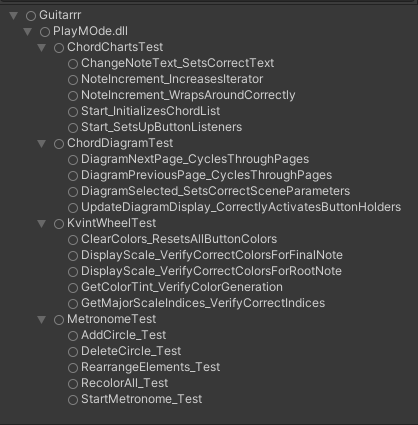
\includegraphics[scale=1]{rys05/Testy}
   \caption{Struktura testów projektu}
   \label{fig:strukturaTestów}
\end{figure}

\subsection{Implementacja testów}

Aby przeprowadzić testy dla poszczególnych komponentów, utworzono mocki (ang.~\emph{mocks} - sztuczne obiekty, udające rzeczywiste zależności). Dla tych obiektów przetestowano działanie poszczególnych funkcji.

\subsubsection{Testy metronom}

Kod przedstawiony na listingu poniżej (listing~\ref{lst:10}), odpowiada za utworzenie sztucznego obiektu \texttt{MetronomeManager}, zawierającego przyciski i pozostałe potrzebne zależności do jego działania. 

\begin{lstlisting}[style=sharpcstyle,caption=Funkcja \texttt{SetupMetronomeManager}, label=lst:10]
private MetronomeManager SetupMetronomeManager()
{
    GameObject gameObject = new GameObject();
    MetronomeManager metronomeManager = gameObject.AddComponent<MetronomeManager>();
    GameObject canvasObject = new GameObject();
    Canvas canvas = canvasObject.AddComponent<Canvas>();
    metronomeManager.canvas = canvas;
    metronomeManager.HigherTempo = CreateMockButton();
    metronomeManager.LowerTempo = CreateMockButton();
    metronomeManager.Begin = CreateMockButton();
    metronomeManager.Add = CreateMockButton();
    metronomeManager.Delete = CreateMockButton();
    ...
    return metronomeManager;
}
\end{lstlisting}

Dla klasy \texttt{MetronomeManager} sprawdzono np.\ funkcję zwiększania i zmniejszania taktu, sprawdzając przy tym, czy poprawnie tworzone są obiekty wchodzące w skład sceny (listing poniżej).

\begin{lstlisting}[style=sharpcstyle,caption=Funkcja \texttt{AddCircle\_Test}, label=lst:20]
[UnityTest]
public IEnumerator AddCircle_Test()
{
    var metronomeManager = SetupMetronomeManager();    
    metronomeManager.AddCircle();
    metronomeManager.AddCircle();
    metronomeManager.AddCircle();
    
    Assert.AreEqual(3, metronomeManager.circles.Count);
    yield return null;
}
\end{lstlisting}

Pozostałe testy obejmowały sprawdzenie poprawności funkcji odpowiedzialnych za dynamiczne rozmieszczanie elementów graficznych an scenie, działanie wątku metronomu, zmianę koloru elementów graficznych sceny, zwiększanie i zmniejszanie bpm.

\subsubsection{Testy koło kwintowe}

Testy jednostkowe koła kwintowego obejmowały utworzenie mocków obiektu głównego menadżera sceny, a następnie zbadanie działania funkcji odpowiedzialnych za zarządzanie przyciskami i elementami graficznymi scen. Na listingach ~\ref{lst:30} i \ref{lst:40} zamieszczono wybrane części kodu odpowiedzialnego za przeprowadzenie testów.

\begin{lstlisting}[style=sharpcstyle,caption=Funkcja \texttt{SetupKvintManager}, label=lst:30]
private KvintManagerScript SetupKvintManager(int outerButtonCount = 12, int innerButtonCount = 12)
{
    GameObject managerObject = new GameObject();
    KvintManagerScript kvintManager = managerObject.AddComponent<KvintManagerScript>();
    
    kvintManager.outerButtons = new List<Button>();
    for (int i = 0; i < outerButtonCount; i++)
    {
        GameObject buttonObject = new GameObject($"OuterButton_{i}");
        Button button = buttonObject.AddComponent<Button>();
        Image buttonImage = buttonObject.AddComponent<Image>();
        buttonImage.color = Color.white;
        kvintManager.outerButtons.Add(button);
    }
    return kvintManager;
}  
\end{lstlisting}

\begin{lstlisting}[style=sharpcstyle,caption=Funkcja \texttt{GetMajorScaleIndices\_VerifyCorrectIndices}, label=lst:40]
[Test]
public void GetMajorScaleIndices_VerifyCorrectIndices()
{
    var kvintManager = SetupKvintManager();
    int rootNoteIndex = 0;
    var scaleIndices = kvintManager.GetType()
        .GetMethod("GetMajorScaleIndices", System.Reflection.BindingFlags.NonPublic | System.Reflection.BindingFlags.Instance)
        .Invoke(kvintManager, new object[] { rootNoteIndex }) as List<int>;

    Assert.IsNotNull(scaleIndices);    
    List<int> expectedIndices = new List<int> { 11, 0, 1, 2, 3, 4, 5};
    CollectionAssert.AreEqual(expectedIndices, scaleIndices);
}
\end{lstlisting}

\subsubsection{Testy księga akordów}

Testy dla księgi akordów skupiały się na testowaniu działania funkcji odpowiedzialnych za zmianę aktualnie wyświetlanego akordu (listing~\ref{lst:60}). Wpierw utworzono sztuczny obiekt (listing~\ref{lst:50}), który następnie poddano testom.

\begin{lstlisting}[style=sharpcstyle,caption=Funkcja \texttt{SetupChordChartsManager}, label=lst:50]
private ChordChartsManager SetupChordChartsManager()
{

    GameObject managerObject = new GameObject();
    ChordChartsManager chordChartsManager = managerObject.AddComponent<ChordChartsManager>();

    GameObject noteTextObject = new GameObject();
    chordChartsManager.noteText = noteTextObject.AddComponent<Text>();

    GameObject variantTextObject = new GameObject();
    chordChartsManager.variantText = variantTextObject.AddComponent<Text>();

    chordChartsManager.SaveButton = CreateMockButton();
    chordChartsManager.noteLeft = CreateMockButton();
    chordChartsManager.noteRight = CreateMockButton();
    ...
    return chordChartsManager;
}
\end{lstlisting}


\begin{lstlisting}[style=sharpcstyle,caption=Funkcja \texttt{NoteIncrement\_WrapsAroundCorrectly}, label=lst:60]
[Test]
public void NoteIncrement_WrapsAroundCorrectly()
{
    var chordChartsManager = SetupChordChartsManager();
    chordChartsManager.noteIterator = 11;
    chordChartsManager.noteIncrement();
    Assert.AreEqual(0, chordChartsManager.noteIterator);

    chordChartsManager.noteDecrement();
    Assert.AreEqual(11, chordChartsManager.noteIterator);
}
\end{lstlisting}

\subsubsection{Testy diagramu akordów}

Dla głównego menadżera sceny diagramu akordów utworzono sztuczny obiekt wraz ze sztucznie utworzonymi elementami graficznymi i przyciskami, sprawdzając, czy przy przewijaniu diagramu dezaktywowane i aktywowane są odpowiednie elementy sceny. Przykłady kodu źródłowego zamieszczono na listingach (listing~\ref{lst:70}, \ref{lst:80}). Dodatkowo testowano poprawne ustawienie klasy odpowiedzialnej za komunikację pomiędzy scenami diagramu akordów i księgi akordów.

\begin{lstlisting}[style=sharpcstyle,caption=Funkcja \texttt{Setup}, label=lst:70]
[SetUp]
public void Setup()
{
    gameObject = new GameObject();
    chordDiagram = gameObject.AddComponent<ChordDiagram>();

    SetupMockComponents();
}
\end{lstlisting}

\begin{lstlisting}[style=sharpcstyle,caption=Funkcja \texttt{DiagramNextPage\_CyclesThroughPages}, label=lst:80]
[Test]
public void DiagramNextPage_CyclesThroughPages()
{
    Assert.AreEqual(0, chordDiagram.currentIndex);

    chordDiagram.DiagramNextPage();
    Assert.AreEqual(5, chordDiagram.currentIndex);

    chordDiagram.DiagramNextPage();
    Assert.AreEqual(10, chordDiagram.currentIndex);

    chordDiagram.DiagramNextPage();
    Assert.AreEqual(0, chordDiagram.currentIndex);
}
\end{lstlisting}